%% This template is based on the sample-acmtog template from overleaf.

%% The first command in your LaTeX source must be the \documentclass command.
\documentclass[acmtog, nonacm]{acmart}

%% \BibTeX command to typeset BibTeX logo in the docs
\AtBeginDocument{%
  \providecommand\BibTeX{{%
    \normalfont B\kern-0.5em{\scshape i\kern-0.25em b}\kern-0.8em\TeX}}}

\setcopyright{none}

%%\acmSubmissionID{123-A56-BU3}

%%
%% For managing citations, it is recommended to use bibliography
%% files in BibTeX format.
%%
%% You can then either use BibTeX with the ACM-Reference-Format style,
%% or BibLaTeX with the acmnumeric or acmauthoryear sytles, that include
%% support for advanced citation of software artefact from the
%% biblatex-software package, also separately available on CTAN.
%%
%% Look at the sample-*-biblatex.tex files for templates showcasing
%% the biblatex styles.
%%

%%
%% The majority of ACM publications use numbered citations and
%% references.  The command \citestyle{authoryear} switches to the
%% "author year" style.
%%
%% If you are preparing content for an event
%% sponsored by ACM SIGGRAPH, you must use the "author year" style of
%% citations and references.
\citestyle{acmauthoryear}

\usepackage{tikzducks}
%%
%% end of the preamble, start of the body of the document source.
\begin{document}

%% The "title" command has an optional parameter,
%% allowing the author to define a "short title" to be used in page headers.
\title{Baking a great loaf of bread.}
\subtitle{Group Report for COMP5530}

%% The "author" command and its associated commands are used to define
%% the authors and their affiliations.
%% Of note is the shared affiliation of the first two authors, and the
%% "authornote" and "authornotemark" commands
%% used to denote shared contribution to the research.
\author{Rafael Kuffner dos Anjos}
\authornote{Sharing first authorship}
\email{r.kuffnerdosanjos@leeds.ac.uk}
\author{Nina Ambulance}
\authornotemark[1]
\email{ninanina@leeds.ac.uk}
\author{Amanda Lynn}
\authornotemark[1]
\email{musician@leeds.ac.uk}
\author{Lipin Jection}
\authornotemark[1]
\email{smooch@leeds.ac.uk}
\author{Rhoda Camel}
\authornotemark[1]
\email{yeehaw@leeds.ac.uk}
\author{Robyn Banks}
\authornotemark[1]
\email{oceans11@leeds.ac.uk}
\author{Anita Bath}
\authornotemark[1]
\email{bathtime@leeds.ac.uk}
\affiliation{%
  \institution{University of Leeds}
  \streetaddress{Woodhouse}
  \city{Leeds}
  \state{West Yorkshire}
  \country{United Kingdom}
  \postcode{LS2 9BW}
}

\author{Shaunper Vysier}
\email{shaunpervysier@leeds.ac.uk}
\affiliation{%
  \institution{University of Leeds}
  \country{United Kingdom}}
\additionalaffiliation{the role of Supervisor}

  
%% By default, the full list of authors will be used in the page
%% headers. Often, this list is too long, and will overlap
%% other information printed in the page headers. This command allows
%% the author to define a more concise list
%% of authors' names for this purpose.
%\renewcommand{\shortauthors}{Dos Anjos, et al.}

%%
%% The abstract is a short summary of the work to be presented in the
%% article.
\begin{abstract}
  \textcolor{blue}{This section here is the abstract, which is a summary of your work in no more than \textbf{150 words}.}
  Bread is one of the oldest prepared foods in history.
  A staple across many cultures in our blue planet, it can be ingested in any meal one desires. 
  While many purchase their loafs weekly from supermarkets, it is not always the smartest choice. 
  Mold, bread's biggest nemesis can conquer your slices if they are left on the counter top for too long, making their consumption an uninviting prospect. 
  In this project we describe the ancient process of baking a loaf of bread from water and flour, covering a few little variants.
  We show that our loaf is tasty, as it was consumed in less than two hours, and discuss possible improvements for our future baking endeavours.  
\end{abstract}

%%
%% The code below is generated by the tool at http://dl.acm.org/ccs.cfm.
%% Please copy and paste the code instead of the example below.
%%
\begin{CCSXML}
<ccs2012>
   <concept>
       <concept_id>10003752.10003809.10010052</concept_id>
       <concept_desc>Theory of computation~Parameterized complexity and exact algorithms</concept_desc>
       <concept_significance>100</concept_significance>
       </concept>
   <concept>
       <concept_id>10010583.10010750</concept_id>
       <concept_desc>Hardware~Robustness</concept_desc>
       <concept_significance>300</concept_significance>
       </concept>
   <concept>
       <concept_id>10010147.10010371.10010396.10010401</concept_id>
       <concept_desc>Computing methodologies~Volumetric models</concept_desc>
       <concept_significance>500</concept_significance>
       </concept>
 </ccs2012>
\end{CCSXML}

\ccsdesc[100]{Theory of computation~Parameterized complexity and exact algorithms}
\ccsdesc[300]{Hardware~Robustness}
\ccsdesc[500]{Computing methodologies~Volumetric models}

%%
%% Keywords. The author(s) should pick words that accurately describe
%% the work being presented. Separate the keywords with commas.
\keywords{bread, yeast, baking, food}

\received{20 February 2007}
\received[revised]{12 March 2009}
\received[accepted]{5 June 2009}

%Teaser figure. Optional to have in the beginning of your paper if you have a great image for your project. 
\begin{teaserfigure}
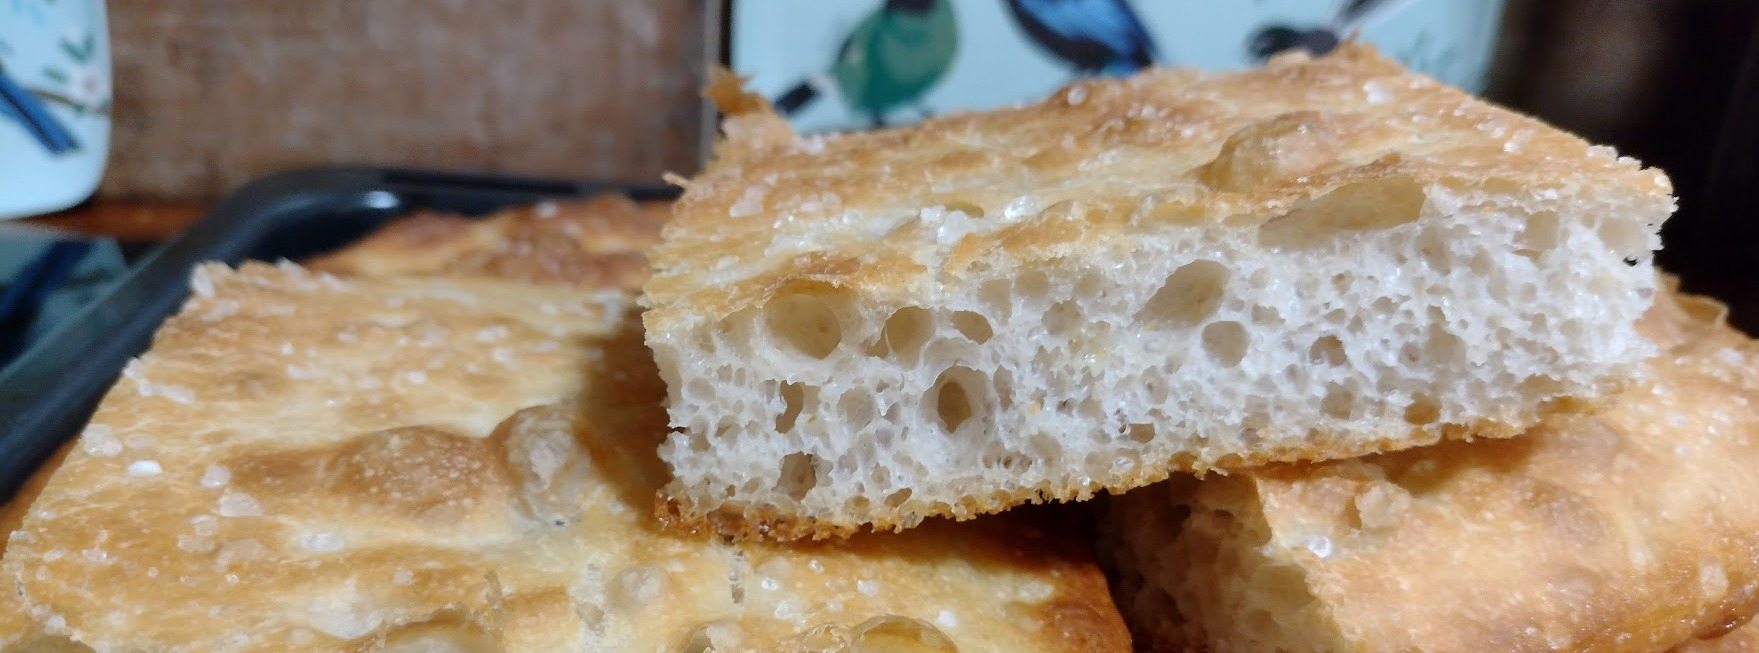
\includegraphics[width=\textwidth]{focaccia}
\caption{Italian type of bread: Focaccia. Tasted really nice with butternut squash soup.}
\label{fig:teaser}
\end{teaserfigure}

%%
%% This command processes the author and affiliation and title
%% information and builds the first part of the formatted document.
\maketitle

%%
\section{Introduction}
\textcolor{blue}{The introduction of your report must give the reader some context, motivation for choosing this as a project, describing what you did, and giving a sneak peak of your results.
This works as a way of getting someone to read the rest of the paper, almost like a pitch.
The whole report should be no more than 12 pages, references and figures included. 
4 Pages are reserved for project management on the appendix. }

The popular saying ``the greatest thing since sliced bread'' has made its way into our vocabulary in 1928 \cite{slicedBread} pushing the previous greatest thing into obscurity.
This list of greatest things can be tracked through the lighbulb (1880), the telegraph (1830), the steam engine (1720), and all the way to the original greatest: bread itself. 

Bread has been traced down to the most ancient human civilizations \cite{OldBread}, most likely due to its preparation consisting of very basic ingredients combined together; flour and water. 
In fact, it has been listed in accounts from early civilizations as basic nourishment side by side with water \cite{slicedBread,Bible}.
One is left to wonder how did this marvelous invention came about, and who has been this unsung hero who ground some grains, mixed them with water until sticky, and heat it in fire. 
Regardless if a stroke of luck, genious, divine inspiration, or alien technology, this method exist, and variations on it have been developed, as seen in Figure \ref{fig:teaser}. 

During the recent SARS-CoV-2\footnote{more popularly known as ``the rona''} pandemic, people had a lot of free time.
While some started working out, or cutting their own hair, a large amount of home-dwellers started exploring the ancient art of baking bread, in order to avoid catching the rona at the supermarket, resorting to their unethical stockpile of flour in their pantries. 
Resorting to youtube, pintrest, and blogs with longer than necessary backstories in the marriage of whoever wrote the recipe, people ended up giving up on this hobby altogether. 


In this project, our group will be baking a great loaf of bread, in a nice to read scientific manner so future bakers can use it as a guide.
Our recipe is perfect for lazy people, as it minimizes the attention you need to give to the loaf, allowing you to binge watch TV shows without guilt. 
Our results were considered to be above average, and can be ingested with a variety of toppings.
This report will provide some background detail on the art of making bread, followed by a clear description of our method, evaluation of results, and discussions about how our method can be expanded to different types of loafs. 


\section{Background Research}
\label{sec:background}
\textcolor{blue}{Your background research should include a detailed review of known industry/academic work, and how they relate to what you want to do.
It should not be simply a list of papers/methods with a short description about them.
Instead, it should put them in context, establishing relationships, differences, highlights, limitations, and ultimately relating them to your proposed work. 
You should not need to explain concepts that are already known by the reader. 
The readers for your project will be academic staff at this university, so while there are some concepts that are important to introduce, you do not need to explain what a computer is. 
Remember the old saying: Don't preach to the choir.
Overall, this section should allow readers to understand what people in this field have been doing.}

Bread making involves the transformation of flour, water, and other ingredients into a porous and palatable product through the combined action of physical, chemical, and biological processes.
The main factors that affect the quality and characteristics of bread are the type and composition of flour, the choice and amount of leavening agent, the kneading and shaping of dough, the fermentation and proofing conditions, and the baking parameters \cite{breadchemistry}. 

\subsection{Ingredients}

Classic bread is made of flour and water. 
Wheat flour contains starch and protein.
When mixed with water, the protein forms gluten, which is a network of elastic molecules that gives bread its squishy texture and volume. 
The amount of gluten depends on the type of flour used, and other factors which will be discussed later. 
Some people are intolerant to gluten, an auto-immune disorder called the celiac disease.
Complications may range from diarrhea to cancer and death. 
Thus, other flours can also be used in the fabrication of bread, such as rice flour or tapioca flour, giving it a different taste, texture, and elasticity.
It has been noted by casual observers that it is more difficult to achieve a squishy loaf without gluten. 

Leavening agents can be used to produce carbon dioxide in your bread and make it expand. 
They can be chemical (baking soda or powder) or biological (yeast), the most popular option for bread.
It is important to mention that "unleavened bread" is in some cultures the most popular option, such as tortillas in mexico, matzo, piadinas, and roti. 

Salt is important to add to your bread, as it adds flavour.
Fine salt is normally mixed with the dough, even for sweet breads that take sugar in their recipes.
Focaccia, notably, takes extra coarse salt on top of the bread.

Some oil can be added to breads, introducing some fat content to it. 
It is widely known that fat can make some foods tastier. 

Finally, eggs and milk are a crucial ingredient to one of the most delicious breads ever invented, the brioche. 
While it was unclear to this group what its role is in the process as we are computer scientists and not bakers, its success is undeniable.


\subsection{Processes}

Breadmaking has developed with several methods being introduced to increase the quality of loaves. 
Kneading is the first one. 
After mixing the ingredients properly, you should fight with the dough using your hands in order for the gluten molecules to develop. 

One popular method is the stretch and fold. 
You pull one end, fold it to the center, rotate the dough, and repeat it.
Another one is the fold and punch, normally used when you have a bowl, and pent-up anger. 
This is closely related to the stretch and slam, where you lift the dough, stretch it, and slam on the countertop while grunting in frustration about your general life. 
All of these methods require a resting time for both the dough and yourself, to allow the gluten to develop, and for you to deal with your emotions. 
It has been reported that having your hands either wet or full of flour make this process a little bit less sticky to the fingers. 

\begin{figure}
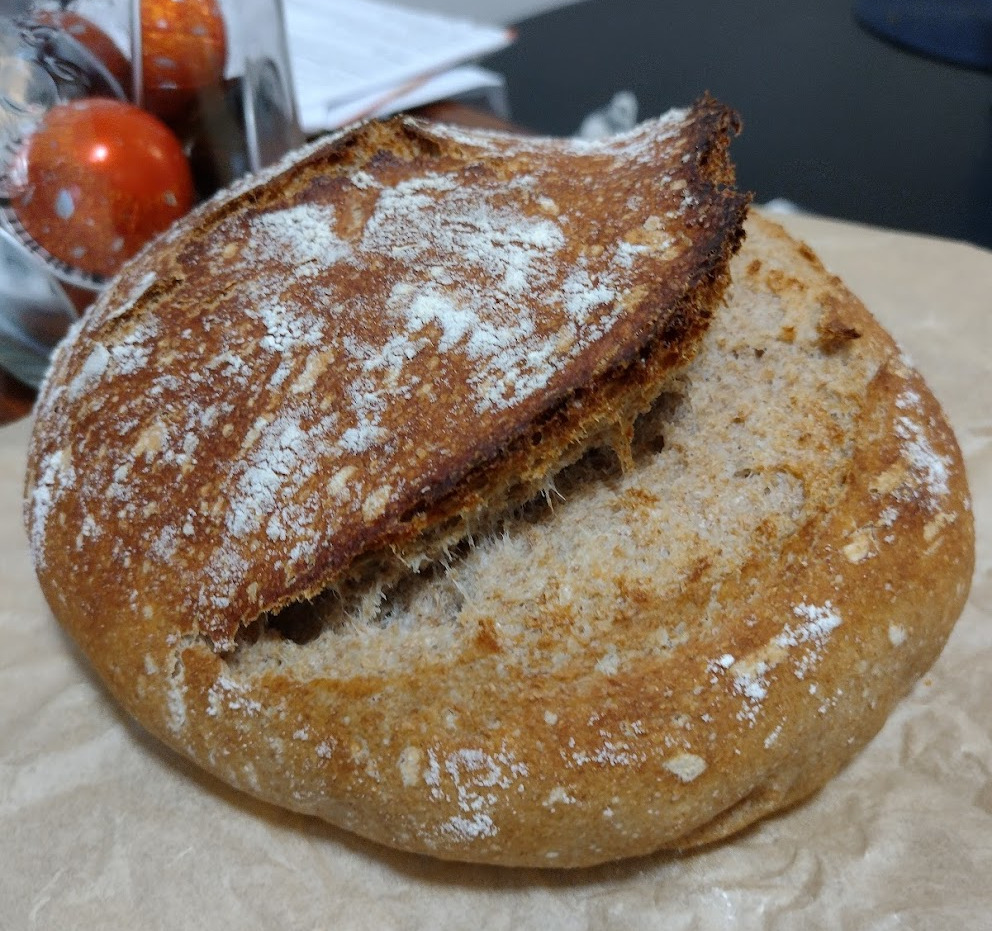
\includegraphics[width=\columnwidth]{scoring.jpg}
\caption{Result of scoring the loaf before baking. The crust lifts allowing the rest of the loaf to grow.}
\label{fig:scoring}
\end{figure}

Fermentation is the stage where the leavening agent consumes the sugars in flour and produces carbon dioxide gas and other by-products, such as alcohol, organic acids, and aroma compounds.
It normally happens at room temperature or a controlled environment, for varying lengths of time, depending on the type of bread, and the length of the TV show you are watching. 
While the risk of overproofing your bread, aka forgetting about it, exists, its \textbf{damages} when in the United Kingdom are low, due to low average temperatures of kitchens. 

Baking is how the ingredients go from sticky goo to edible sponge.
By heating the mixture up to high temperatures, chemical reactions \cite{breadchemistry} take care of the process of making your dreams come true. 
During this process, more fermentation may happen, producing more CO2, and allowing your bread to expand even more. 
It is widely known that cutting shapes on the top of the bread (an art known as scoring) may allow its center to expand further, creating a bigger loaf, and a prettier one for you socials as seen in Figure \ref{fig:scoring}. 
Time and temperature will vary with the type of bread you are making \cite{breadchemistry}, with some loaves taking just 15 minutes, and others a full hour in the oven. 

\subsection{Summary}
There is way too much to know about bread, and way too many options. 
Flours, yeast, shaping, the unknown impact of new york water in the quality of bagels, it is all overwhelming.
We focused our efforts in creating the perfect recipe for the lazy, leaving the more complicated loaves for future work. 

\section{Method}

\begin{figure*}[h]
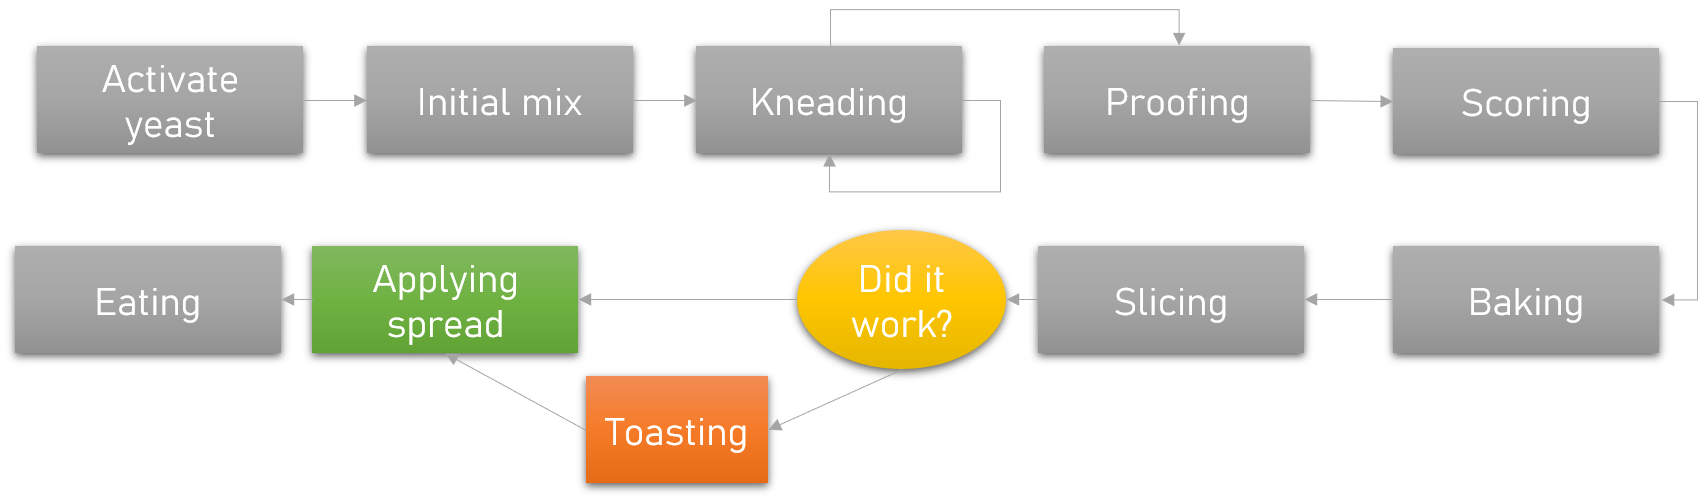
\includegraphics[width=\textwidth]{diagram.png}
\caption{Overview of our method. It always ends with the bread being successfully ingested.}
\label{fig:diagram}
\end{figure*}


\textcolor{blue}{Here is where your work should be explained.
The main challenge is finding how granular your descriptions should be. 
While it is tempting to talk about everything and have 89 pages of going through every single class in your code, nobody will be terribly excited about reading it. 
Remember who your target audience is: people with interest in knowing how you achieved this.
You can expect that they either know how some things work, or can probably figure it out by themselves. 
The question normally asked about this section of the work is: "could this method be reproduced by a motivated student based on this description?", which for your case, can be reworded as "could another group read our report, and re-implement what we did just based on what we described?".
Ask for help from your supervisor to know what is essential here, as this will vary a lot from the type of project you are implementing.} 

Considering existing popular ingredients and methods for breadmaking, the variation on approaches, time available, the lack of experience of the general bread maker, and the time available to do it properly, we devised the following process described in Figure \ref{fig:diagram}. 
It is an iterative method with one single looping instruction, and a 100\% rate of consumption of the produced loaf, due to an intelligent if statement which corrects for a badly baked bread. 
Our hypothesis are as follows:
\begin{itemize}
    \item H1: A moderately lazy in desperate need of bread can do it.
    \item H2: Resulting loaf results in an audible onomatopoeia of delight after ingested.
\end{itemize}

This section will go through each step in some detail, except for the last step, as ingesting bread is normally a skill acquired around 7 months of age for most humans. 

We will be describing the process used to bake a loaf using 500 grams of flour, as that would be enough for a group that fits in a regular dining room to eat in a controlled manner.
To make the whole process easier, we will be requiring a simple kitchen scale which can be bought from either a local store or global online retailers. 
The full list of ingredients for the loaf is the following:

\begin{itemize}
    \item 500g bread flour
    \item 320g lukewarm\footnote{warm to the touch but not hot} water
    \item 12g salt
    \item 50g of starter / 7g dried yeast
    \item extra flour for other steps. 
\end{itemize}

\subsection{Activate yeast}
Our first ingredient is yeast. 
We will describe two methods used for our loaves.
Both are equally lazy, only depending the availability of ingredients in your local supermarket, or your circle of friends.

\paragraph{Dried Yeast:} If you managed to find this at your local grocery store, buy it.
Sometimes it is not available \footnote{notably absent during the rona season} so pay close attention and store it in your pantry. 
To use it, mix 1 packet (7 grams) with the amount of lukewarm water described in the recipe (see section \ref{sec:initialmix}) and a teaspoon of sugar.
Sugar will allow the yeast start working.
Mix it thoroughly in a big bowl, and leave it resting for five minutes. 
You should see some bubbling happening at the end of this time, which means the yeast has not gone bad.

\paragraph{Sourdough starter:} if you happen to know a millennial or a hipster (they can be both) you can ask for some starter. 
Provide them with a jar, and they will return you some dough in this jar. 
This piece of dough contains ``wild yeast'' captured from the air, and works as a fermenting agent. 
You can also create your own starter capturing the yeast from your place of residence, but this process will not be described here as there is an abundance of millenials and hipsters and we are focusing this method to be as low effort as possible.
To use your starter, take it out of the fridge (the laziest way to store it) the night before you want to bake your bread.
Add 50g of starter to a bowl, together with 25 grams of water and 25 grams of bread flour.
Add 25 grams of water and 25 grams of bread flour back to the starter. 
Mix both of them. 
Starter jar goes back to the fridge, bowl is covered and left at the countertop overnight. 
On the next day, you should see some bubbles in your mixture.
If not, your starter is dead and you should notify your provider. 

\subsection{Initial mix:}
\label{sec:initialmix}

Grab a spoon, salt, scale, lukewarm water, and bread flour.
Depending on how "light" you want the bread to be, the ratio between flour and water is decided. 
Given water W and flour F, hydration can be calculated by $H = \frac{F}{W}$.
The higher the hydration the softer the bread will be, and the stickier the dough will also be. 
It is harder to correctly pull of a wetter loaf for beginners, so after much consideration our group settled on 64\% as it reminded us of a popular edition of a Nintendo console, thus, 320ml or grams, as the density of water makes them mean the same thing. 

Add water to your yeast, mix nicely until it dissolves, then add the flour and salt, and mix everything together with a spoon at first. 
When it becomes obvious your are not making much progress, wash your hands, remove your rings, and use your hands to properly incorporate the ingredients. 
If the ingredients are sticking to your hands, wetting them or coating them in more flour (as mentioned in Section \ref{sec:background}) can prevent some stickiness. 

\subsection{Kneading}
We will be using the popular stretch and fold method. 
After mixing, put a timer on your phone, or start an episode of anime or a sitcom, as those tend to end in roughly 30 minutes. 
When that time is done, wet your hands, grab one side of the dough, stretch it, and fold to the center. Rotate the bowl to complete this four times. 
Cover the dough, put the next episode/timer on, and repeat this process three or four times, depending on how exciting the show is.
If you did it right, the dough is now really stretchy, and it doesnt break apart easily when you pull. 

\subsection{Proofing}
Depending on the time of day where this bread is being produced, there are two different options for proofing your bread. 
If you are tired and want to continue later, stick it in the fridge, and wait to continue on the next day. 
The cold slows down the action from the yeast, while still allowing some growth. 
After that, carry on with what is described here.

Pour flour on a clean counter-top in your living quarters. 
If there is none, use a clean table. 
Pour the mixture on top of the flour, repeat the stretch and fold process one more time, but without rotating the dough.
At the end of it flip it around to have the fold against the hard surface.
Cup your hands like you cup your pet's face when you say ``who's a good doggy'' and use them to shape the dough into a nice ball, pulling it to the sides in order to stretch the top portion a little bit. 
It is important to mention never to punch the dough, as we are not using any of the angry methods in our algorithm, and due to it killing all the bubbles of CO2 our yeast have produced. 
Leave to to rise for half an hour if you just took it off the fridge, or two to four hours if it is the same day. 

\subsection{Scoring}
Grab a good knife, cut the top of the loaf. 
You can optionally try to make some art, but this group has no artistic talent or sharp knives, so we recommend a straight cut down the middle using the tip of your knife. 
It should be enough that you see the dough separating a little bit. 

\subsection{Baking}
Pre-heat your oven to 180\textdegree C, then decide where you are baking this loaf of bread.

If you own a Pirex round casserole, this was found by our group to be the most convenient way of doing it. 
Put baking paper on the lid of the pyrex, and transfer your loaf to it. 
Cover it with the bowl, and stick it in the oven. 
If you have a proper casserole, put the bread inside, and cover with the lid, and stick it in the oven. 
If you down own any type of casserole, put it in a baking tray, or a loaf tin, and cover with aluminum foil try and trap some of the moisture in, as it makes for a crispier loaf. 
If you fail to do this, try adding a second baking tray with some boling water to your oven, as the extra vapours will be helpful to make this work. 

Bake it for 35 minutes covered, then uncover and wait until the crust is golden brown, then remove it from the oven.

\subsection{Slicing}
Wait for the bread to cool down so you avoid burning your hands, or allowing the bread to crumble. 
This is a risky step as you are dealing with a sharp object, and you are also most likely hungry. 

\subsection{Debugging}
One innovative concept of our breadmaking process is the if statement.
If after slicing, a non-spreaded piece is tasted and is considered to be subpar, or the baking was shown to have failed exposing parts of not so well cooked dough inside, or if the whole thing crumbled like one's expectations, sticking it in the toaster always allow for consumption of the loaf. 

\subsection{Applying spread}
Butter was found to be the recommended spread to use on a warm loaf. 
Peanut butter tends to taste better on a slighly cooler slide of bread, as well as jam. 
Nutella works in any way.
Marmite is divisive. 

\section{Evaluation}
\textcolor{blue}{This section should cover how your project was evaluated. 
Regardless of the goal you are trying to achieve, a well designed evaluation should be considered. 
This section should describe what are the components you are trying to evaluate, and how the tests executed were the right ones for the purpose. 
This should be separated from considerations, as you might need to run several separate evaluations, and report distinct set of results that should be considered together. 
Use tables and graphs to communicate your results in an aggregated way, presenting the necessary information for the reader to comprehend your results quickly. 
While you could provide extra data in appendix, all that is necessary for comprehension of your results should be in the body of the report. 
Anyone reviewing your submission should not need to look at appendix to understand a core part of your manuscript. 
The appendix is not a workaround to the page limit, it is a bonus for really interested people. 
A good rule of thumb is: if my appendix is deleted, my report should still be comprehensible. 
}

To validate our two hypothesis H1 and H2, we devised a simple evaluation: baking and tasting. 
If a lazy person was able to produce the loaf, eat it, and say hmmm, both H1 and H2 would be confirmed. 

\subsection{Participants}
While a large scale test with multiple participants was ideal, our time (one afternoon to bake and write this whole joke article) was limited. 
First author was chosen as our designated baker, while the rest of the team observed closely. 
The level of laziness was deemed appropriate for the task, as he notably does not iron his clothes as it is ``too much work''.

\subsection{Methodology}
Ingredients were purchased from the local grocery shop, and baking appliances provided by First author's landlord. 
No help from the team was allowed, but help from family to reach for ingredients, snacking, and mental health support were allowed in order to minimize the impact stress would have on the quality of the loaf. 

\subsection{Results}
\begin{figure}[h]
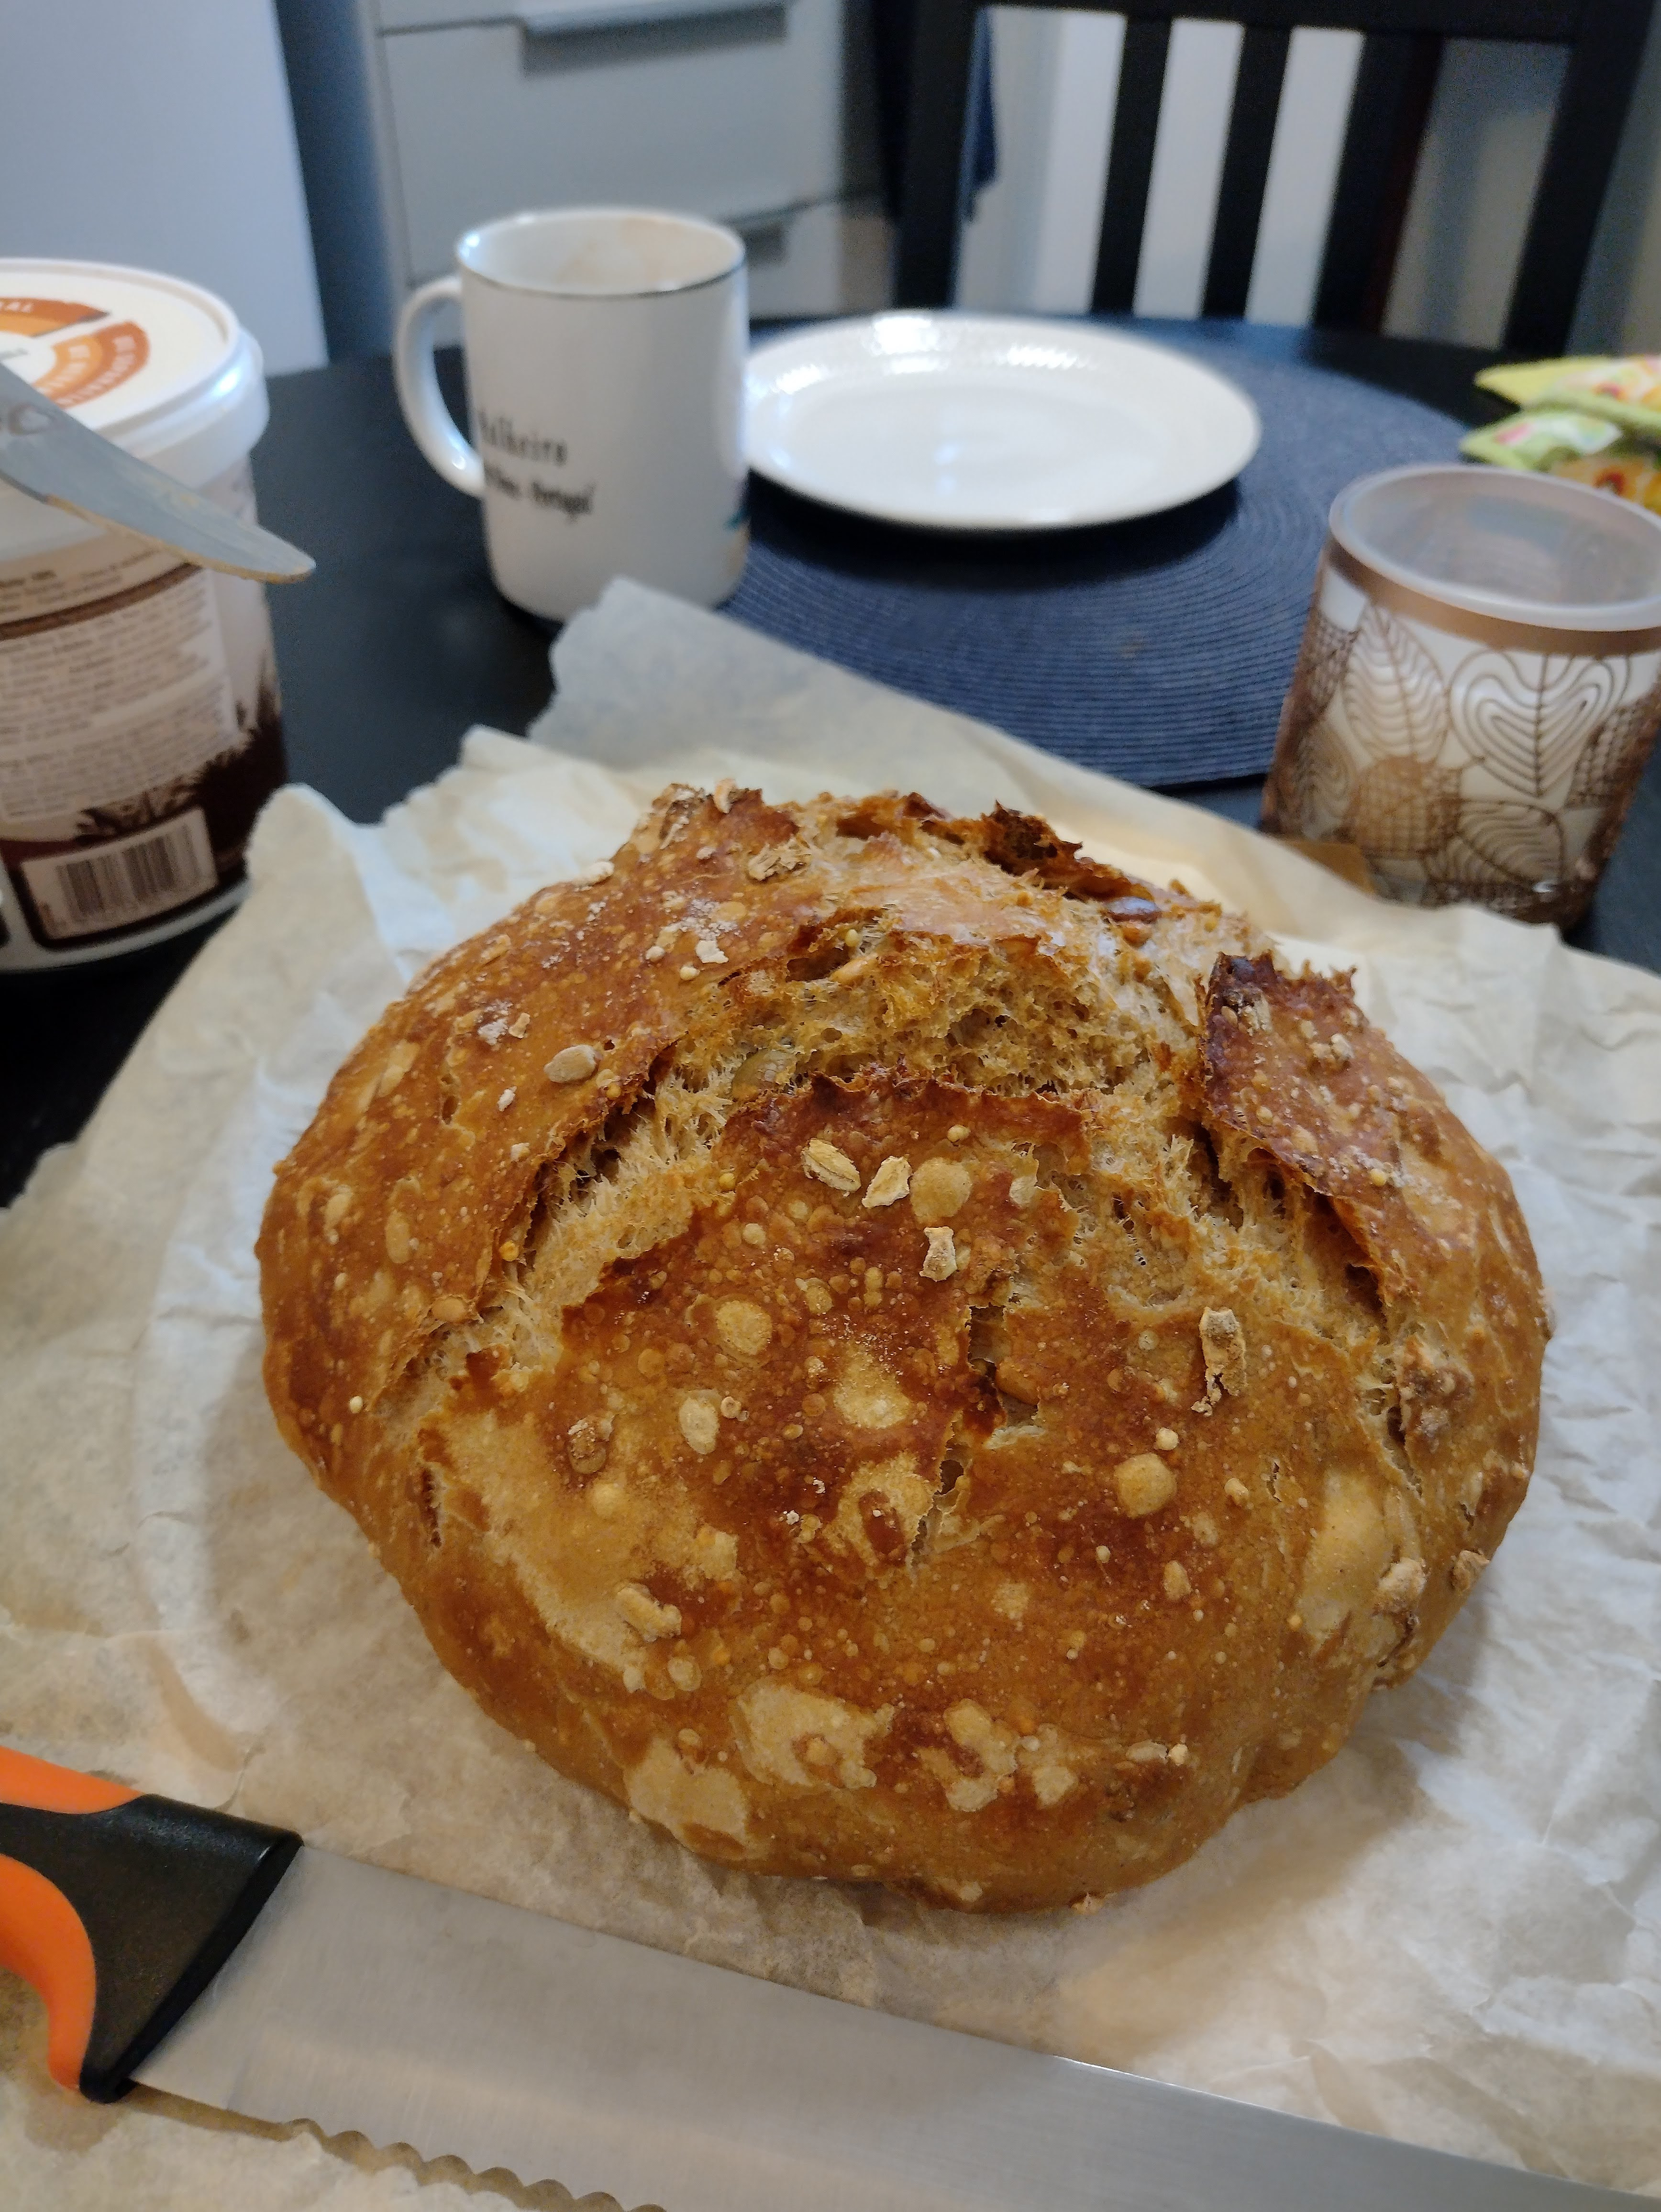
\includegraphics[width=\columnwidth]{goodloaf.jpg}
\caption{A good loaf produced during the evaluation of our method. Peanut butter pictured in the background as the chosen spread.}
\label{fig:goodloaf}
\end{figure}

\begin{figure}[h]
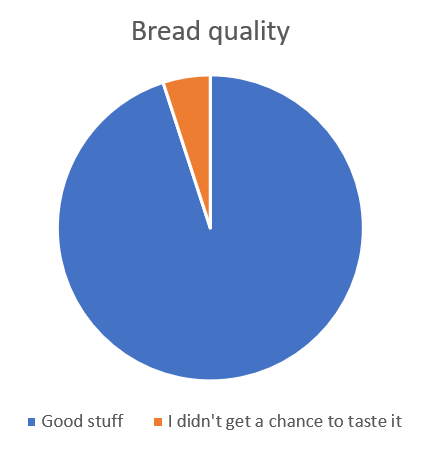
\includegraphics[width=\columnwidth]{piechart.png}
\caption{Overall results of our taste test}
\label{fig:plot}
\end{figure}

Our results can be seen in Figures \ref{fig:goodloaf} and \ref{fig:plot}. 

A successful loaf was achieved on first attempt, with a crispy golden crust. 
During the post-baking interviews, insight on the laziness of the baker and the mental health status after the process was obtained. 
No reports of yelling or crying were found, and two episodes of forgetting the dough was proofing were notified. 
This has had seemingly no impact on the final product. 

Taste test results was overwhelmingly good, with one team member not being able to taste it properly due to delays in getting to the kitchen during tasting time. 

\section{Discussion}
\textcolor{blue}{This is where you actually draw conclusions from your results, and discuss how successful or not things were. 
This is where we would like to see your critical analysis of the method and the results. 
Provide unique insights on why do you think you achieved the results you did in the previous section, do not limit yourself to stating the obvious.}

We found that our results validate both our proposed hypothesis. 
A lazy person was able to produce a loaf that was ingested in rapid fashion.
That is corroborated with the fact that one of the participants did not make it in time for its ingestion. 
We find that the resiliency of the method to forgetting about the loaf multiple times cements it as the go-to way to bake bread if you are afraid of messing up. 

Some work needs to be done with stickiness of hands during folding, as the water method was found to be more suitable, but still not ideal.
The baker added flour to the top of the loaf before baking in an attempt to make it look more ``gourmet''. 
This is a subjective matter that was not conclusively investigated in this experiment, and should be further tested in future work. 

\section{Conclusion}
\textcolor{blue}{Here you draw things to a close.
It should be a much shorter version of your introduction, without the motivation part, but focusing on your results, and what it leads to going forward. 
You can have clear sections for limitations and future work, or work it into the text of your conclusion.}
We have presented a method for lazy breadmaking, which has shown to achieve great success in our evaluation. 
By introducing a lazy stretch and fold mechanism, a ``stick it in the fridge'' option, and a taste-based if statement, we allow zero skill breadmakers to make a competent loaf to save their lives from starvation if they cannot reach the supermarket. 

The main limitation of our method is still requiring to get up and handle ingredients multiple times, but we believe this is the bare minimum a human being should be able to do it, considering podcasts and headphones can be worn during the process. 

In future work we will explore alternative types of bread that can be achieved with a lazy methodology. 
Initial studies show that the Foccacia is a good option, as it trades folding and shaping for more rising time. 
We will be verifying that it is equally lazy to our regular round loaf. 


%%
%% The acknowledgments section is defined using the "acks" environment
%% (and NOT an unnumbered section). This ensures the proper
%% identification of the section in the article metadata, and the
%% consistent spelling of the heading.
\begin{acks}
First author would like to thank his wife for helping pour extra flour when his hands are sticky from dough.
\end{acks}

%%
%% The next two lines define the bibliography style to be used, and
%% the bibliography file.
\bibliographystyle{ACM-Reference-Format}
\bibliography{sample-base}

%%
%% If your work has an appendix, this is the place to put it.
\newpage
\appendix

\section{Project management}
\textcolor{blue}{This is the appendix of your report, which should contain all the project management details, distinct from the scientific content of it. 
Please follow this rough structure, including everything you deem necessary up to the page limit of 6.}

\subsection{Supervisor and Theme}
\textcolor{blue}{Write a short description of how the theme of the project and the supervisor were chosen.
Do not go into long narratives, but this should highlight the good match between the groups interests and the supervisors area of expertise.
Mention how often you had contact with your supervisor, and rough structure of these meetings. 
It should be clear what was their goal. }

\subsection{Group organization}
\textcolor{blue}{What was the adopted development strategy?
How was the group organized? 
Did you have teams?
What are the chosen communication channels? 
How did you organize the code? 
Did you use version control? 
How often did you meet? 
What was the goal of the meetings? 
What measures you had in place to keep everyone in track?
What measures you had in place to ensure deadlines were met?
What measures you had in place to evenly distribute work?}

\subsection{Planning and execution}
\textcolor{blue}{This should contain two gantt charts: the initial planning, and what actually ended up happening.
The text in this section should be a reflection of why there was any different between them, or a reflection on why it was the right choice of planning in case they are exactly the same. }

\section{Self-reflection and soft skills acquired.}
\textcolor{blue}{Overall conclusion of the project from a management point of view. 
Besides the technological and scientific aspects of your project, what did you learn as a group, and how may that be useful in the workforce, hopefully soon? Please provide individual reflections from different group members. Group please make sure what they say is true.}

\section{How ethical issues are addressed}
\textcolor{blue}{This is a University requirement. See Resources on 'Ethics relevant to computing projects' for guidance and discuss it with your supervisor. If no ethical issue is involved, a sentence to that effect will suffice.}

\end{document}
\endinput
%%
%% End of file `sample-acmtog.tex'.
